\documentclass[a4paper, 11pt]{article}
\usepackage{psfrag,amsbsy,graphics,float,amsmath}
\usepackage[english]{babel}

\usepackage{wrapfig}
\usepackage{verbatim} 
\usepackage{bm}
\usepackage{amssymb}
\usepackage{booktabs}
\usepackage[hidelinks]{hyperref} 
\usepackage{natbib}
\usepackage{pdfpages}
\usepackage[toc,page]{appendix}

\usepackage[english]{babel}
\usepackage{blindtext}

\usepackage[capitalise]{cleveref}  
\usepackage{subcaption}

\usepackage{listings}
%%\usepackage{minted}


%---------------------------------------------------------------------------------
% Additional settings
%---------------------------------------------------------------------------------

%---------------------------------------------------------------------------------
% Define your margins
\usepackage{geometry} % Necessary package for defining margins

\geometry{
	top=2cm, % Defines top margin
	bottom=2cm, % Defines bottom margin
	left=2.2cm, % Defines left margin
	right=2.2cm, % Defines right margin
	includehead, % Includes space for a header
	%includefoot, % Includes space for a footer
	%showframe, % Uncomment if you want to show how it looks on the page 
}

\setlength{\parindent}{15pt} % Adjust to set you indent globally 

%---------------------------------------------------------------------------------
% Define your spacing
\usepackage{setspace} % Required for spacing
% Two options:
\linespread{1.5}
%\onehalfspacing % one-half-spacing linespread

%----------------------------------------------------------------------------------------
% Define your fonts
\usepackage[T1]{fontenc} % Output font encoding for international characters
\usepackage[utf8]{inputenc} % Required for inputting international characters

%%\usepackage{XCharter} % Use the XCharter font
\usepackage[font=small,labelfont=bf]{caption}


%---------------------------------------------------------------------------------
% Define your headers and footers
\setlength{\headheight}{14pt}
\usepackage{fancyhdr} % Package is needed to define header and footer
\pagestyle{fancy} % Allows you to customize the headers and footers

%\renewcommand{\sectionmark}[1]{\markboth{#1}{}} % Removes the section number from the header when \leftmark is used

% Headers
\lhead{} % Define left header
\chead{\textit{}} % Define center header - e.g. add your paper title
\rhead{} % Define right header

% Footers
\lfoot{} % Define left footer
\cfoot{\footnotesize \thepage} % Define center footer
\rfoot{ } % Define right footer

%----------------Commands--------------------------
\newcommand{\bp}[2]{\bm{#1(}#2\bm{)}}

%---------------------------------------------------------------------------------

\begin{document}
\setcounter{page}{1}
\thispagestyle{empty}

\includepdf[pages=1,pagecommand={}]{titlepage/titlepage.pdf}

\begin{abstract}
Conspiracy theories are spreading. Especially during the COVID-19 pandemic. To get a
deeper understanding about the impact of those theories we use machine learning techniques
to predict whether a text has high  influence in the conspiracy theory audience. Using 
CrowdTangle, a tool to crawl posts made on Facebook, we create two datasets containing 
posts from conspiracy theorists. We define a metric to measure the impact a post has and
let two models based on neural networks predict this variable for  each post. A brief
insight of explainability methods - which can be used to make a  complex neural
model comprehensible for humans - is given. In this case this could help to understand 
how posts with high impact look like.
\end{abstract}

%_________TOC__________________________
\tableofcontents
\newpage

%_________Introduction__________________________________
%!TEX root = ../main.tex
\section{Introduction}
\label{sec:introduction}
2020 was a challenging year from many perspectives especially because of the COVID19
pandemic.  As a study from Cambridge shows conspiracy theories about this topic are rising
everywhere \citep{freeman_waite_etal_2020}. These theories can be  dangerous, as one can
conduct from the Capitol riot in the United States January 6th, 2021. At this event,
people believed in a conspiracy theory that Trump's victory in the US elections 2020 was 
stolen from him and tried therefore to ``take it back'' by storming the US
Capitol~\citep{williamson_2021}. They organized this riot on a social media platform. The 
question is: How can we fight conspiracies like that? A first step could be to try to 
understand how conspiracy theories work in the context of social media.  Why do certain
theories get shared? With the help of Natural Language Processing (NLP) and machine
learning we analyzed posts written by conspiracy  theorists in order to find answers  to
the following questions: can we predict the impact of a conspiracy theory post using the 
post's content? How do we define impact? Can we give an explanation on what makes a post 
successful or unsuccessful among conspiracy theorist? While NLP and neural networks can be
used to process text and assign a label to it, often it is to hard for humans to
understand how they came to a certain conclusion. The field of eXplainable Artificial 
Intelligence (XAI) tries to give explanations about why machine learning models make a 
specific prediction.  If we only have a model which predicts the impact of a social media
post, we still do not  know how the model came to this decision. With XAI we can reason
about it - or more  importantly: we can reason about what a successful post might look
like and thus identify what stances conspiracy theorists support. 

% Edo: global XAI could be used to understand social groups and posts impact within those groups. So you reviewed global XAI methods, you tried to predict posts impact on crowdtangle, and future work should focus on the combination if they find good data that is predictable
% \begin{itemize}
%     \item Similar to the extended abstract
%     \item Introduction to the topic of XAI 
%     \item General methodology
% \end{itemize}
%!TEX root = ../main.tex
\section{Related Work}
\label{sec:related_work}

\citet{guidotti2018survey} gave a fundamental overview of the current research in XAI: 
\emph{Model explanation} and \emph{outcome explanation} are two of four 
categories defined by them. These are also know as
\emph{global} and \emph{local} explainability. Approaches of the local category try to
give an  instance-level explanation. Thus we only consider one or a small group of samples
and reason about the model's classification for them. On the other hand, approaches which 
belong to the global category try to explain the model as a whole, i.e. if we have several
output categories, how does a typical input look like for one output category. All papers
which were analyzed by \citet{guidotti2018survey} which fall into the outcome explanation
category use  some kind of surrogate model. The surrogate is usually a simpler,
human-comprehensible model  (e.g. a linear model or a decision tree), which tries to
imitate the complex one. The  trade-off is the precision. All models in this category work
on tabular data, except the one from \citet{krishnan2017palm} which is independent of the
data's format. 

\citet{Lundberg_2017} came up with an explainability framework based on Shapley values for 
local explainability. In 2020 they proposed a new Shapley value based framework called
SAGE for the model explanation problem~\citep{NEURIPS2020_c7bf0b7c}. While the first one
could easily be applied to natural  language, the second one might not. For images, they
combined several pixels to a so-called \emph{super pixel} in order to save computations, i.e.
only the impact of a superpixel is  measured. One idea to use SAGE for  textual data
could be to apply the same idea to text. While pixel at a certain location inside an image 
might give a hint to a certain outcome, a word's position inside a text usually does not 
have such an impact. Words or sentences are usually location independent. This means we 
can not explain outcomes by just looking at the n-th word of a text. In regards of
text a superpixel has to be represented by a fragment of text, e.g. a named entity or another closed 
unit which is only dependent on whether it is included in the text at all rather than the 
precision position of it inside the text.

% \begin{itemize}
%     \item Overview of global XAI methods which have been done so far \citep{guidotti2018survey} 
%     \begin{itemize}
%         \item short overview of different categories
%         \item lack of explainability methods for text based data
%     \end{itemize}
%     \item SAGE \citep{NEURIPS2020_c7bf0b7c}
%     \begin{itemize}
%         \item Basic introduction of this paper
%         \item Difficulties when using it for natural language
%     \end{itemize}
%     \item Brief summary of other papers which I had a look at (wiki) \dots 
% \end{itemize}

%_________Main Content__________________________________
%%%!TEX root = ../main.tex
\section{Background}
\label{sec:background}

%!TEX root = ../main.tex
\section{Dataset}
\label{sec:dataset}
We built our custom dataset and created  definitions for the success of a post in order to
answer the following research questions: \emph{What makes a text successful  among
conspiracy theorists?}, \emph{What are the keywords making a post get the most  attention
from this kind of audience?}.  In this section, we describe how we retrieved posted  text
from conspiracy theorists on Facebook, how we analyzed these posts and define our own 
metric for \emph{impact}.

\subsection{Data Retrieval}
We built our own dataset using posts from Facebook. We gathered these posts using 
CrowdTangle\footnote{https://crowdtangle.com}, ``a public insights tool owned and operated
by Facebook''~\citep{ctshiffmanciting}. While having some limitations this tool lets us 
find posts by specifying keywords. Our goal was to create a dataset containing posts of 
conspiracy theorists. Besides searching posts including a keyword, one can choose between
posts of a Facebook group or posts of a Facebook page. Crowdtangle only supports groups
which are public (i.e. every Facebook  users can read the posts of the group and join it
without an invitation) and have over 2000 members. One can also exclude posts, group names
or page names containing a certain word. We wanted the dataset to contain at least 30,000 posts to be able to used in deep neuronal network as they require more training
data as simpler models. In order to achieve this, two problems had to be tackled. First we
had to choose wisely which keywords to include in our search. Second we needed to find
actual conspiracy theory discussion groups instead of ones posting ironic content. As these
pages and groups share false information, they are a deletion target of Facebook. We
chose a popular video containing wrong information and clearly had conspiracy
theorists as target audience for our search. We then crawled for posts which shared this video.
Using the downloaded list we extracted the groups these posts belonged to. In CrowdTangle we
sorted these groups by their total interaction count in the last month.  Facebook offers
 to react to a post by clicking on an emoji, writing a comment or by sharing the post 
with others. A post  with a lot of
interaction was usually seen by more people and thus was more important. Groups with more
interactions in total are more active and usually had more members than groups with fewer
interactions. Choosing groups with high interaction counts has two advantages. First we
gain more posts for a given time span than from groups with lower interaction counts in
the same time span. Second the posts themselves have usually more individual interactions.
Using this sorted list we handpicked ten groups (a list of names can be found in
Figure~\ref{fig:dataset-group-names}) of which we were sure are groups run by actual
conspiracy theorists and not just sharing conspiracy theories ironically. 

Along with the conspiracy group dataset, we collected a second dataset consisting of
post from Russia Today's Facebook page (rtnews). Russia Today is known for  publishing
false information and conspiracy theories as shown by \citet{yablokov2015conspiracy}. 

\subsection{Dataset description}
\label{subsec:dataset:description}
For both datasets we decided to only include posts which were at least two months old. The
 idea behind this was that as a post gets older it moves down in the timelime of a group
or  page. The further down a post moves the less attention it receives. With posts being
over two months old, the chances are higher that the interaction count will not change
much over time. Naturally there are exceptions: for example an old post could be shared
on a very popular page. Then this  post might see a strong increase in interactions even
if it is older than two months. This is a limitation resulting from our decision. 

Among others we get following features for each post: post type (can be one of \emph{Link},
\emph{Native Video}, \emph{Photo}, \emph{Status}, \emph{Video}, \emph{YouTube}), number of
interactions (\emph{Likes}, \emph{Comments}, \emph{Shares}, \emph{Love}, \emph{Wow},
\emph{Haha}, \emph{Sad}, \emph{Angry}, \emph{Care}), message, link (points to the shared
video or link), image text (for  post type \emph{Image}, Facebook uses
OCR\footnote{optical character recognition} to extract  text which is displayed in the
image), link text, description and total interactions.

\subsection{Data Preprocessing} The preprocessing consisted of two steps. 
\begin{enumerate} 
    \item We removed posts with duplicate content. In our Facebook group dataset this is
more likely  as different members might share the same content more than once. On the other
hand, for
Facebook pages  this is rather unlikely as the rtnews page is run by a single
organization which coordinates all published posts. We considered a post as a duplicate
if the message and image text were equal. For the rtnews set we considered a post
being a duplication if message, link text, image text and description were equal. 
    \item We created our own score variable which we tried to predict later and added it to
each row of the dataset. A detailed description of this variable can be found in a  later
part of this section. 
\end{enumerate}
For rtnews this resulted in a removal of only 1\% of the posts. These posts happened to
have no message,  image text, link text and description at all. At the end we were left
with 57,650 posts. For the group dataset 52\% of the posts were duplications, leaving us
with 33,638 posts. 
\begin{figure}[tb] 
    \centering
    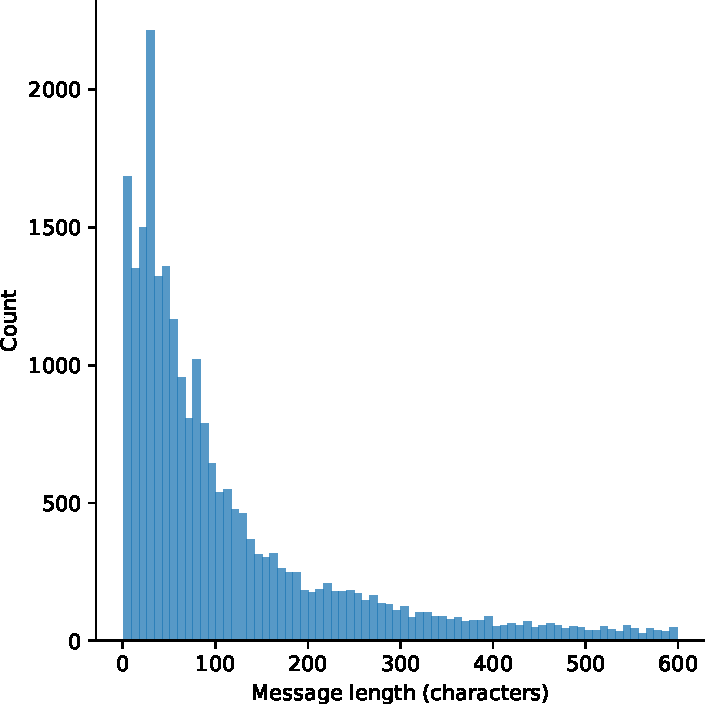
\includegraphics[width=.32\textwidth]{figures/dataset_groups/message_length_dist.pdf}
    \raisebox{-0.7cm}{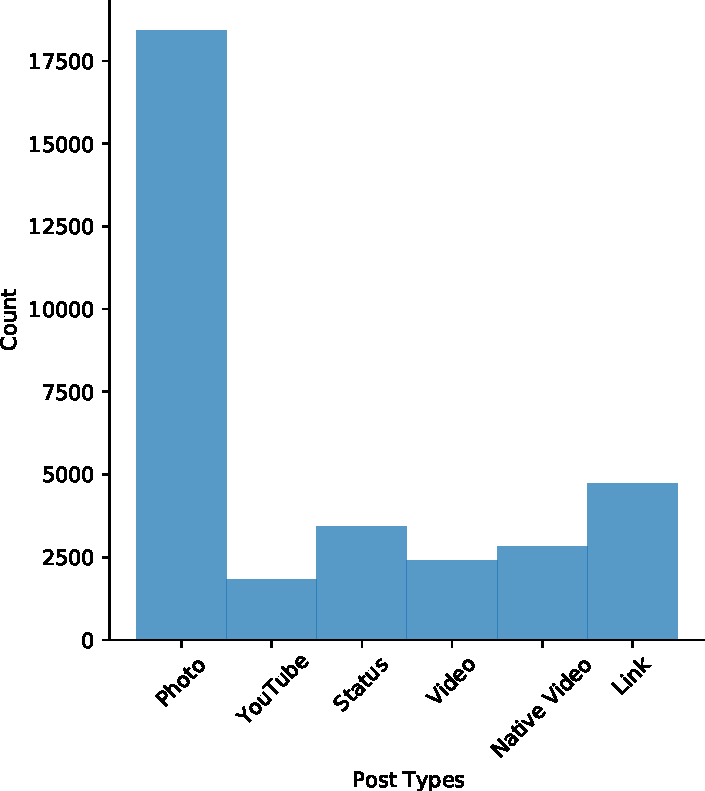
\includegraphics[width=.32\textwidth]{figures/dataset_groups/post_types_dist.pdf}}
    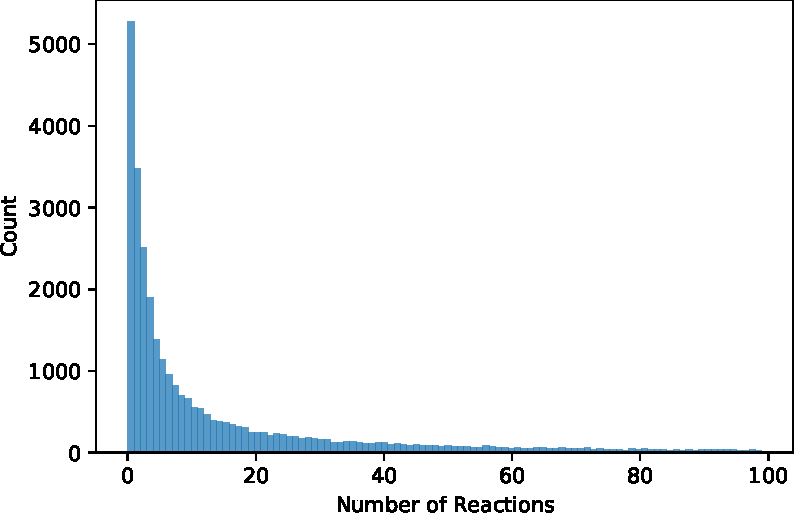
\includegraphics[width=.32\textwidth]{figures/dataset_groups/reactions_dist.pdf}
    \caption{Facebook Conspiracy Theory Group Dataset}
    \label{fig:datasetstats-groups}
\end{figure} 
\begin{figure}[tb] 
    \centering
    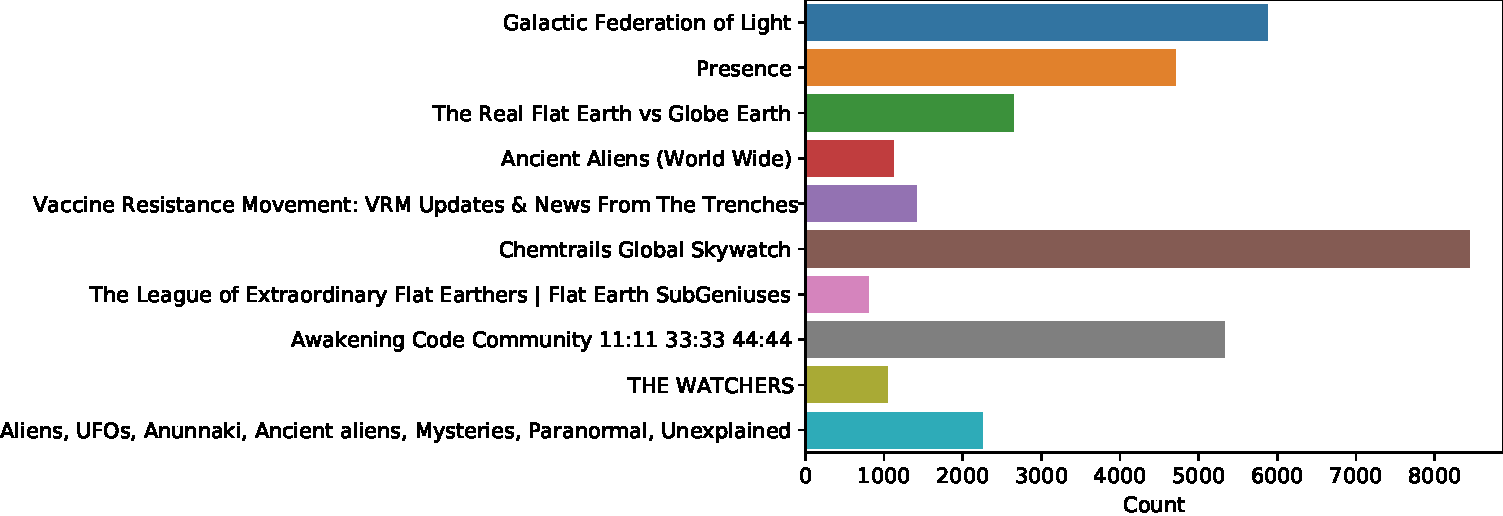
\includegraphics[width=\textwidth]{figures/dataset_groups/group_dist.pdf}
    \caption{Facebook Conspiracy Theory Groups}
    \label{fig:dataset-group-names}
\end{figure}
Figure~\ref{fig:datasetstats-groups} shows the distribution of message length, post type 
and number of reactions for the group dataset. Most messages were below 500 characters and
got less than 20 reactions. As Facebook  already provided us with the text extracted from
images, the high amount of image post  was no issue for us. As mentioned before, we
already removed all duplicate posts. If no text could be  extracted from the image and the
message was the same, the post would have already been removed as part of the preprocessing.
As the number of group members influences the number of reactions, we tried to overcome
the unequal distribution of groups (Figure~\ref{fig:dataset-group-names}) by including the
group's ID as a feature for our models. 
\begin{figure}[tb] 
    \centering
    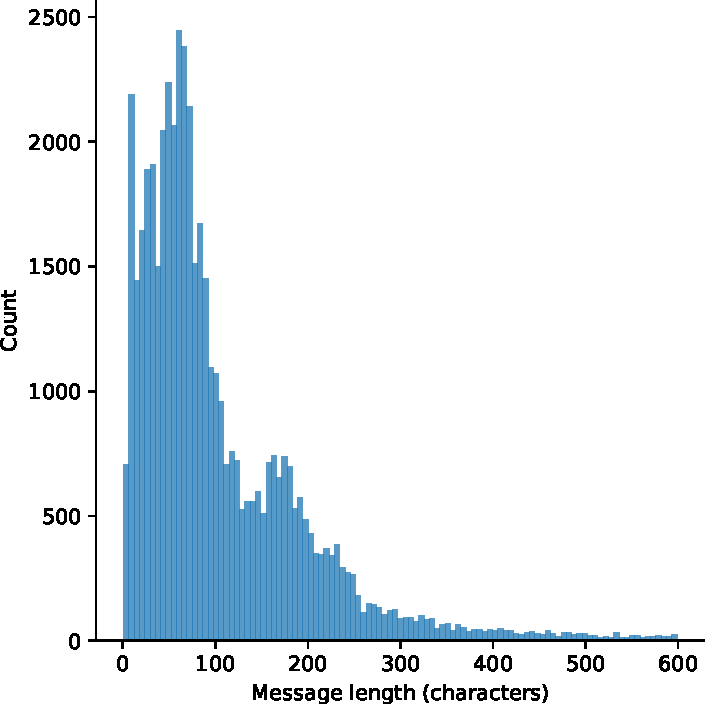
\includegraphics[width=.28\textwidth]{figures/dataset_rtnews/message_length_dist.pdf}
    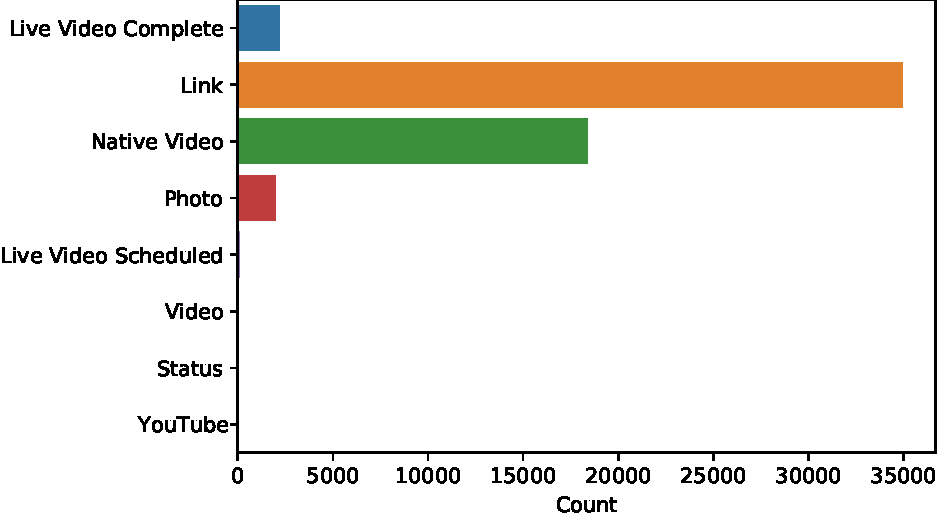
\includegraphics[width=.40\textwidth]{figures/dataset_rtnews/post_types_dist.pdf}
    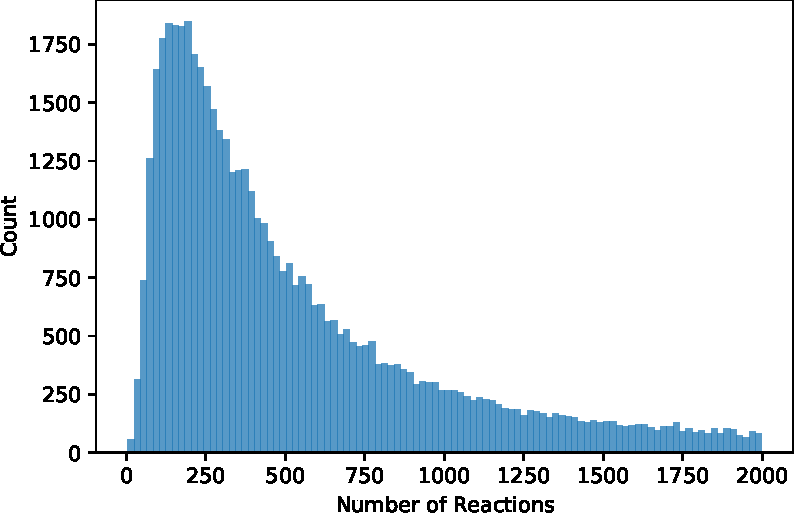
\includegraphics[width=.30\textwidth]{figures/dataset_rtnews/reactions_dist.pdf}
    \caption{rtnews Dataset}
    \label{fig:datasetstats-rtnews}
\end{figure} 
In contrast to the group dataset which consisted of heterogeneous posts made by a large
variety of users, the rtnews dataset only contained post of a single entity's Facebook 
page. Figure~\ref{fig:datasetstats-rtnews} gives some insights. The average message length
is longer. While the group dataset's most used post type was \emph{Photo} the most used type
for rtnews was \emph{Link}. As rtnews is a global television network, most of their posts
link to their own website. Most posts of the group dataset got no reactions at 
all. For rtnews the peak is about around 150 reactions per post.

\subsection{Dependent Variable}
We wanted to use this dataset to predict how much impact a post might achieve in a
specific group. A post has high impact if it gets more reactions as the average post of a 
group. We defined the set of posts for each Facebook group $G$ as follows
\[
    P_G = \{p_1, \dots, p_n\}
\]
with $p_1, \dots, p_n$ being individual posts. We can retrieve the sum of all kinds of
reactions that a specific post $p_i$ got by calling $r(p_i)$. First we calculated the average
number of reactions a post gets for each group  individually:
\[
    \tilde{p}_G = \frac{1}{n} \sum_{p_i \in P_G} r(p_i)
\]
The dependent variable we wanted to predict is a ratio of the post's reaction count and
the  average reaction count a post gets in a certain group $G$:
\[
    y(p_i) = \frac{r(p_i)}{\tilde{p}}
\]
For the rtnews dataset we assumed that we only have a single group and thus the dependent 
variable would only be the ratio of a post's reaction count and the average reaction count
inside rtnews.
%% - A post might get less attention if it goes down the timeline 
%%   => we only picked old posts
%% - picked a time range such that we get > 30,000 posts
%% - CT limitations max x posts...
%% \begin{itemize}
%%     \item Introduction to CrowdTangle
%%     \item Overview of our datasets (rtnews and conspiracy groups).
%%     \begin{itemize}
%%         \item How the data was collected
%%         \item Statistics/graphs explaining the datasets
%%     \end{itemize}
%%     \item Explanation of the conducted preprocessing
%%     \item Our score variable, description of the formula and the reasoning behind it
%% 
%%     \item Description of our task (i.e. predicting the impact of a post inside a group)
%%     \item Benefits which can be gained from this task (i.e. What triggers the success of 
%%     a post inside a certain group/echo chamber? How can one describe an usual post from a 
%%     certain group?)
%% \end{itemize}
%!TEX root = ../main.tex
\section{Experiments}
\label{sec:experiments}
We started with defining a simple linear model as baseline and then created two  models
based on neural networks. In this section we explain the models' structure. Then the
setup of the  experiment will be described and in the end, we show the performance of our
models.

\subsection{The Baseline Model}
\label{subsec:experiments:baselinemodel}
We chose a linear regression model from scikit-learn \citep{scikit-learn} as our baseline. As
features we only used the categorical variables \emph{group}, \emph{post type} and \emph{top level 
domain}. The post types were already listed in section~\ref{subsec:dataset:description}.
The top level domain was extracted whenever a link was attached to the post. For the training 
dataset we ended up with 886 different top level domains. All categorical features were 
one-hot-encoded. The text of the post was omitted for the linear model.


\subsection{Neural Network based on DistilBert} 
\label{subsec:experiments:distilbertmodel}
The first model using neural networks was based on DistilBert \citep{sanh2020distilbert}.
We used the Python library \emph{transformers} \citep{wolf-etal-2020-transformers} which 
comes with a pre-trained tokenizer and vocabulary. The DistilBert model was used to
process text resulting from the concatenation of a post's \emph{message}, \emph{image text}, 
\emph{link text} and \emph{description}. In order to let the network process the categorical
features from section~\ref{subsec:experiments:baselinemodel} they were one-hot-encoded,
and then input in a one layer network.  The output of both was concatenated and finally
processed through a linear layer with the output size of one. Only rectified linear units
were used as non linearities. Adam~\citep{DBLP:journals/corr/KingmaB14} was used as
optimizer.

\subsection{BiLSTM based Model} 
\label{subsec:experiments:bilstmmodel}
The second neural model was based on a BiLSTM and used a similar structure to the
DistilBert one.  While the BiLSTM was responsible for the textual features, the
categorical ones were processed by a  one layer neural network followed by a concatenation
of the BiLSTM's output which  then was processed by a single linear layer. Adam~\citep{DBLP:journals/corr/KingmaB14} was used as the optimizer for this model as well.

\subsection{Experiment Setup}
\label{subsec:experiments:setup}
We used a 60-20-20 split for the train, validation and testset. The metric we used to 
measure the performance was the mean squared error (MSE). For the models based on neural
networks, we tried different learning rates manually. 

\subsection{Results}
\label{subsec:experiments:results}
\begin{table}[tb]
    \caption{mean squared error for all models and datasets}
    \label{tab:results-all}
    \centering

    \begin{tabular}{l|l|l}
    \hline

    \hline
    & \textbf{conspiracy theory groups} & \textbf{rtnews}\\
    \hline
    linear model & 6.68 & 177.51\\
    \hline
    DistilBert & 6.46 & 177.00\\
    \hline
    BiLSTM & 6.54 & 177.44\\
    \hline
    \end{tabular}
\end{table}
\begin{table}[tb]
    \caption{mean squared error for each group}
    \label{tab:result-mse-per-group}
    \centering
    \begin{tabular}{l|l|l|l}
        Group & Linear Model & DistilBert based & BiLSTM \\
        \hline
        \hline
        Galactic Federation of Light & 12.71 & 12.49 & 12.58\\
        Presence & 3.51 & 3.39 & 3.46\\
        The Real Flat Earth vs Globe Earth & 2.18 & 2.16 & 2.07\\
        Ancient Aliens (World Wide) & 2.08 & 1.90 & 1.94\\
        Vaccine Resistance Movement VRM Updates \dots & 5.43 & 5.24 & 5.47\\
        Chemtrails Global Skywatch & 7.10 & 7.00 & 6.99\\
        The League of Extraordinary Flat Earthers \dots & 1.22 & 0.84 & 0.95\\
        Awakening Code Community 1111 3333 4444 & 7.75 & 7.42 & 7.61\\
        THE WATCHERS & 2.21 & 2.01 & 2.12\\
        Aliens, UFOs, Anunnaki, Ancient aliens, \dots & 6.72 & 5.97 & 6.21\\
    \end{tabular}
\end{table}
The lowest error was achieved by the neural model based on DistilBert with an MSE of 6.46
for the conspiracy theory group dataset and an MSE of 177 for the rtnews dataset. The 
results can be found in Table~\ref{tab:results-all}. In
Table~\ref{tab:result-mse-per-group} the MSE was calculated on a per group basis for the
conspiracy theory group dataset. The lowest error was achieved for the \emph{The League of
Extraordinary Flat Earthers | Flat Earth SubGeniuses} group's posts using the DistilBert
model with an MSE of 0.84.
\begin{figure}[tb]
    \centering
    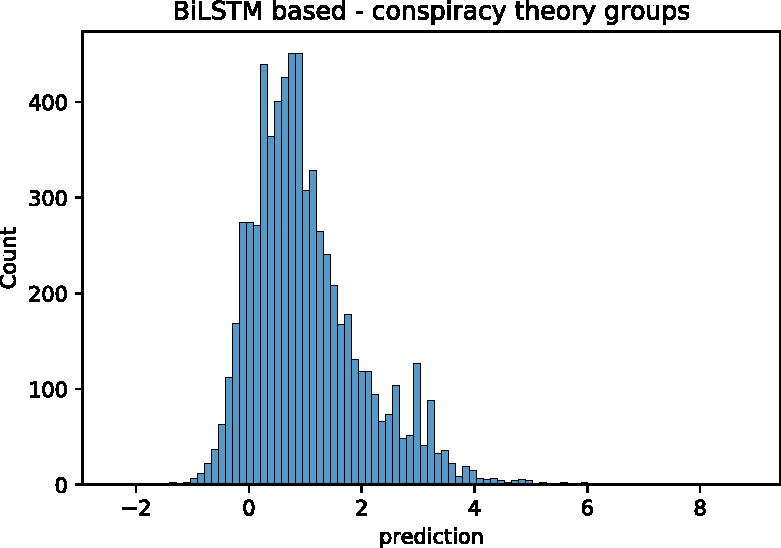
\includegraphics[width=.33\textwidth]{figures/prediction_groups/bilstm_dist.pdf}
    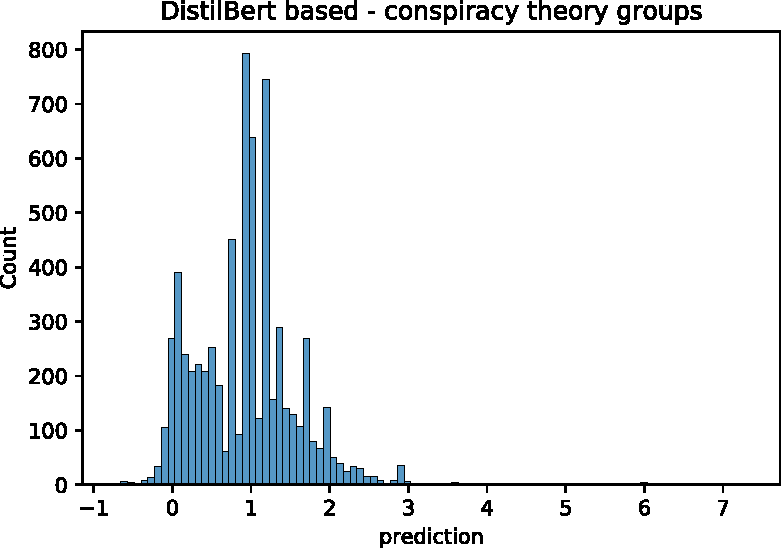
\includegraphics[width=.32\textwidth]{figures/prediction_groups/distil_bert_dist.pdf}
    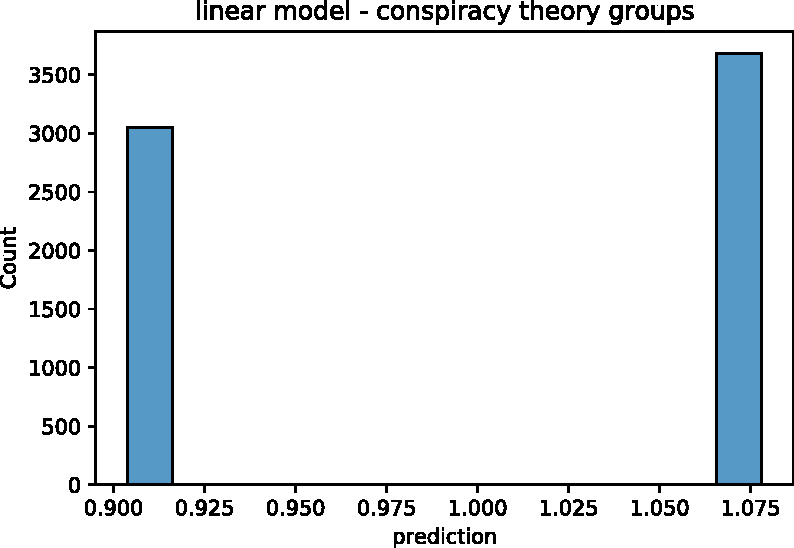
\includegraphics[width=.33\textwidth]{figures/prediction_groups/linear_model_prediction_dist.pdf}
    \caption{distribution of the model's score variable prediction for the conspiracy theory group dataset}
    \label{fig:dist-prediction-groups}
\end{figure}
\begin{figure}[tb]
    \centering
    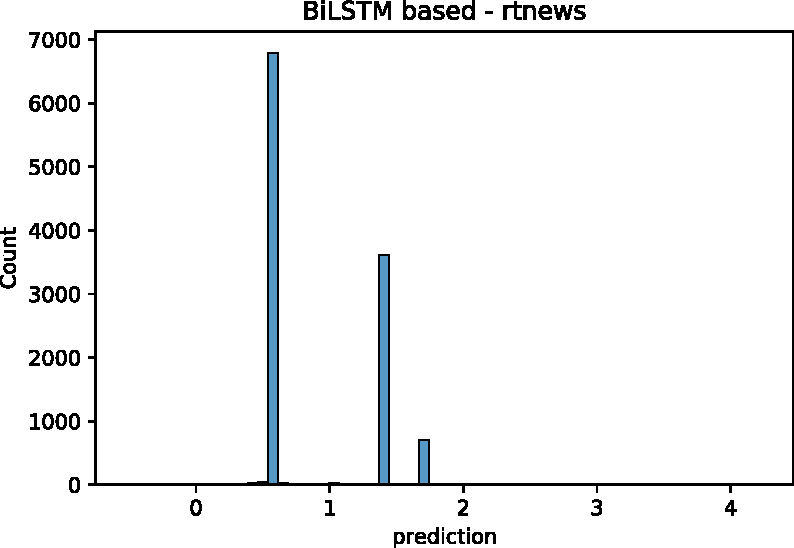
\includegraphics[width=.33\textwidth]{figures/prediction_rtnews/bilstm_dist.pdf}
    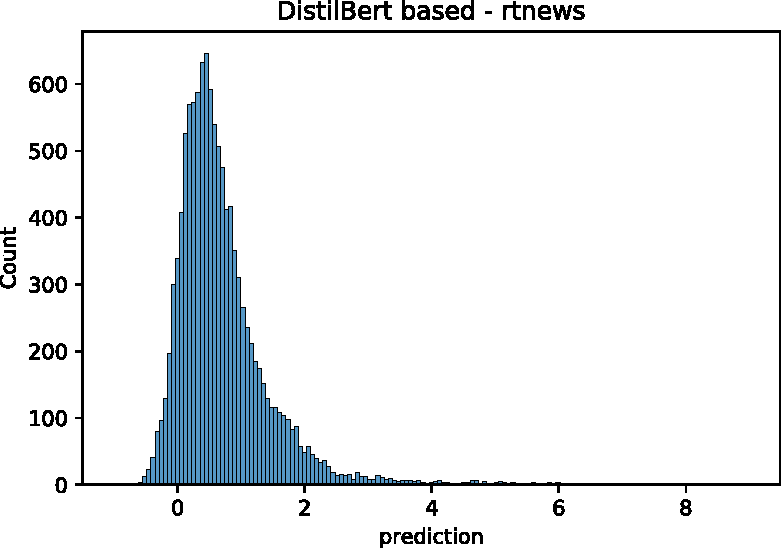
\includegraphics[width=.32\textwidth]{figures/prediction_rtnews/distil_bert_dist.pdf}
    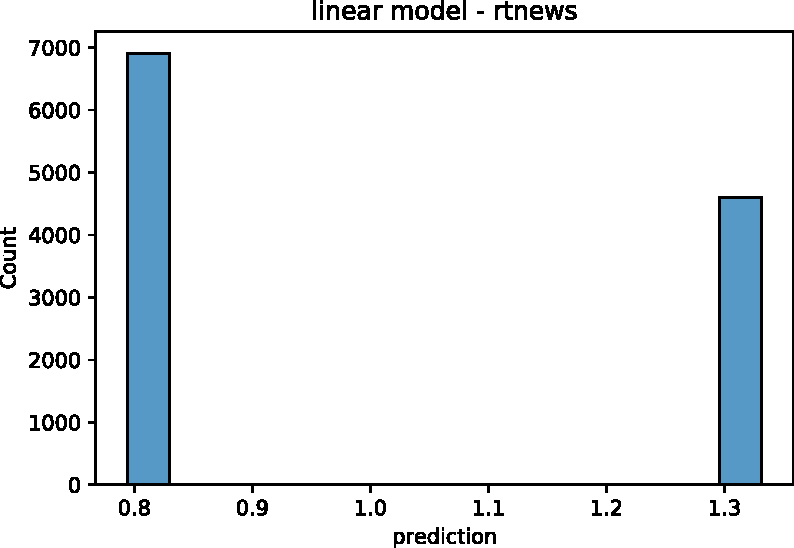
\includegraphics[width=.33\textwidth]{figures/prediction_rtnews/linear_model_prediction_dist.pdf}
    \caption{distribution of the model's score variable prediction for the rtnews dataset}
    \label{fig:dist-prediction-rtnews}
\end{figure}
The histograms of the models predictions can be seen in Figure~\ref{fig:dist-prediction-groups}
for the conspiracy theory group dataset and in Figure~\ref{fig:dist-prediction-rtnews} for 
the rtnews dataset. We assume that the linear model predicted an average based on one of 
the categorical variables (e.g. post type).

 

%_____Discussion, Conclusion_________________________________

%!TEX root = ../main.tex
\section{Discussion, Limitations and Conclusion}
\label{sec:conclusion}
Unfortunately our neural models did not outperform the linear one significantly. 
The linear model is already transparent by design, as the feature weights 
represent directly the influence an input feature has on the result. As we mentioned in
Section~\ref{sec:related_work}, linear models are already used as surrogate for more 
complex models as they are comprehensible for humans. Thus, we did not do any work on 
explainability as our linear model has good performance and could be used as a surrogate
for  the deep neural ones.

We were hoping to find patterns inside a post's text which lead to higher or lower
reaction counts. As the  linear model only considered categorical features and scored
similar performance, this was  not the case. 

The overall higher error of the rtnews dataset can be explained with the dataset's score 
distribution. Rtnews has a higher variance of their posts' score
(Figure~\ref{fig:datasetstats-rtnews}) in comparison to the conspiracy theory group dataset
(Figure~\ref{fig:datasetstats-groups}). 

With only two peak score values as prediction (Figure~\ref{fig:dist-prediction-groups}),
the  linear model almost performed as good as the neural ones. This could be circumvented
by  a more balanced dataset with a uniform distribution of the post reactions count. The
other aspect regarding the dataset is the selection of post sources. We decided to pick
posts  from groups having conspiracy theories as their topic. The relation between score and 
reaction count could behave different in groups or pages with other topics (e.g.
politics).

With the current setup, we could not proof a relation between a post's text and the number
of reactions. There might be no relation at all but we would like to give an idea on what
could still be tried but was not conducted due to time constraints. Facebook  groups
consist of a heterogeneous mix of individuals and most of the posts might not get  much
attention at all (Figure~\ref{fig:datasetstats-groups}). One approach could be to  focus
more on Facebook pages. We only conducted this experiment on a single Facebook page. This
path could lead to more promising results and is yet to be explored.

% \begin{itemize}
%     \item Summarize the insights we obtained
%     \item Problems:
%     \begin{itemize}
%         \item Score variable may not be dependent on the post's text itself
%         \item Unbalanced dataset
%         \item Posts inside groups vary a lot (e.g. off-topic posts vs. viral topic)
%     \end{itemize}

% \end{itemize}


%_____Future Work_________________________________
%!TEX root = ../main.tex
% \section{Future Work}
% \label{sec:future_work}
% \begin{itemize}
%     \item Propose changes in the dataset (more balanced data)
%     \item Try to predict something else (e.g. topic, stance) which offers opportunities 
%     to do global XAI.
%     \item Show some possibilities the datasets have to offer.
% \end{itemize}


%_____References_________________________________
%%\newpage
\bibliographystyle{abbrvnat}
\bibliography{library}
\addcontentsline{toc}{section}{Bibliography} 

%__________________________________________________________
\end{document}
